\subsubsection{Swarm MAG data products}

\begin{verbatim}
import datetime
import matplotlib.pyplot as plt
import numpy as np
import pathlib
import os

import geospacelab.visualization.mpl.dashboards as dashboards

cwd = pathlib.Path(os.path.abspath(''))
file_dir_figure = cwd / 'figures'
file_dir_figure.mkdir(parents=True, exist_ok=True)
\end{verbatim}

\paragraph{Swarm MAG LR data}

\subparagraph{Overview with a long time span}

\begin{verbatim}
def test_swarm_MAG_LR_overview():
    """Test Swarm MAG LR data product
    
    """
    dt_fr = datetime.datetime(2016, 3, 14, 12, 0)
    dt_to = datetime.datetime(2016, 3, 15, 23, 59)

    db = dashboards.TSDashboard(
        dt_fr=dt_fr, dt_to=dt_to, figure_config={'figsize': (8, 12)},
        )

    ds = db.dock(datasource_contents=['esa_eo', 'swarm', 'l1b', 'mag_lr'], sat_id='A', add_APEX=True,)

    panel_layouts = [
        [ds['F']],
        [ds['B_N'], ds['B_E'], ds['B_C']],
        [ds['B_VFM_x'], ds['B_VFM_y'], ds['B_VFM_z']],
        [ds['dB_Sun_VFM_x'], ds['dB_Sun_VFM_y'], ds['dB_Sun_VFM_z']],
        [ds['dB_AOCS_VFM_x'], ds['dB_AOCS_VFM_y'], ds['dB_AOCS_VFM_z']],
        [ds['dB_other_VFM_x'], ds['dB_other_VFM_y'], ds['dB_other_VFM_z']],
        [ds['FLAG_F_BIN_AUX']],
        [ds['FLAG_B_BIN_AUX']],
        [ds['FLAG_q_BIN_AUX']],
        [ds['FLAG_Platform_BIN_AUX']],
    ]

    db.set_layout(panel_layouts=panel_layouts)
    db.draw()
    db.add_title(title='Swarm -{} MAG LR Overview'.format(ds.sat_id), fontsize='medium', append_time=True)

    db.save_figure(
        file_dir=file_dir_figure, 
        file_name='example_MAG_LR_Swarm -{}_overview'.format(ds.sat_id), 
        dpi=100, 
        append_time=False
    )
    db.show()
test_swarm_MAG_LR_overview()
\end{verbatim}

\begin{verbatim}
Create a new figure: Figure(800x1200).
\end{verbatim}

\begin{verbatim}
Load IGRF coefficients ...
\end{verbatim}

\begin{verbatim}
Searching the data product "MAG_LR" with the version "latest" on the server...
The file [PosixPath('/data/afys -ionosphere/data/ESA/SWARM/Level1b/MAG_LR/0701/Sat_A/2016/SW_OPER_MAGA_LR_1B_20160314T000000_20160314T235959_0701_ASM_VFM_IC.cdf'), PosixPath('/data/afys -ionosphere/data/ESA/SWARM/Level1b/MAG_LR/0701/Sat_A/2016/SW_OPER_MAGA_LR_1B_20160314T000000_20160314T235959_0701_MDR_MAG_LR.cdf')] already exists: skip downloading.
The file [PosixPath('/data/afys -ionosphere/data/ESA/SWARM/Level1b/MAG_LR/0701/Sat_A/2016/SW_OPER_MAGA_LR_1B_20160315T000000_20160315T235959_0701_MDR_MAG_LR.cdf'), PosixPath('/data/afys -ionosphere/data/ESA/SWARM/Level1b/MAG_LR/0701/Sat_A/2016/SW_OPER_MAGA_LR_1B_20160315T000000_20160315T235959_0701_ASM_VFM_IC.cdf')] already exists: skip downloading.
WARNING: Multiple files found for the pattern *20160314T000000*20160314T235959*0701*.cdf in the directory /data/afys -ionosphere/data/ESA/SWARM/Level1b/MAG_LR/0701/Sat_A/2016!
WARNING: Multiple files found for the pattern *20160315T000000*20160315T235959*0701*.cdf in the directory /data/afys -ionosphere/data/ESA/SWARM/Level1b/MAG_LR/0701/Sat_A/2016!
/opt/anaconda3/envs/Swarm/lib/python3.12/site -packages/numpy/_core/numeric.py:476: RuntimeWarning: invalid value encountered in cast
  multiarray.copyto(res, fill_value, casting='unsafe')
\end{verbatim}

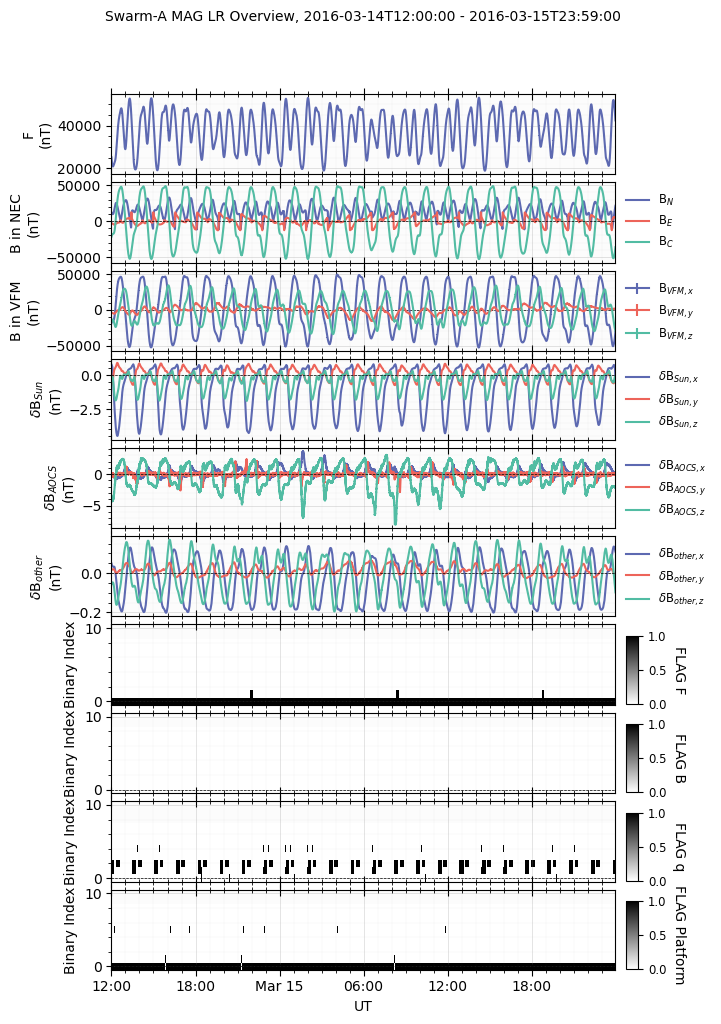
\includegraphics[width=0.7\linewidth]{files/12be9de16ba06b3da42497f3e3204f8d.png}

\subparagraph{Zoomed-in view with a short time span}

\begin{verbatim}
def test_swarm_MAG_LR_zoom():
    """Test Swarm MAG LR data product
    
    """
    dt_fr = datetime.datetime(2016, 3, 15, 18, 18)
    dt_to = datetime.datetime(2016, 3, 15, 18, 23)

    db = dashboards.TSDashboard(
        dt_fr=dt_fr, dt_to=dt_to, figure_config={'figsize': (8, 12)},
        timeline_extra_labels=['GEO_LAT', 'GEO_LON', 'APEX_LAT', 'APEX_LON', 'APEX_MLT',]  # Not applicable for very scattered data points like AEJ_PBS peaks
        )

    ds = db.dock(datasource_contents=['esa_eo', 'swarm', 'l1b', 'mag_lr'], sat_id='A', add_APEX=True,)

    panel_layouts = [
        [ds['F']],
        [ds['B_N'], ds['B_E'], ds['B_C']],
        [ds['B_VFM_x'], ds['B_VFM_y'], ds['B_VFM_z']],
        [ds['dB_Sun_VFM_x'], ds['dB_Sun_VFM_y'], ds['dB_Sun_VFM_z']],
        [ds['dB_AOCS_VFM_x'], ds['dB_AOCS_VFM_y'], ds['dB_AOCS_VFM_z']],
        [ds['dB_other_VFM_x'], ds['dB_other_VFM_y'], ds['dB_other_VFM_z']],
        [ds['FLAG_F_BIN_AUX']],
        [ds['FLAG_B_BIN_AUX']],
        [ds['FLAG_q_BIN_AUX']],
        [ds['FLAG_Platform_BIN_AUX']],
    ]

    db.set_layout(panel_layouts=panel_layouts)
    db.draw()
    db.add_title(title='Swarm -{} MAG LR Zoom'.format(ds.sat_id), fontsize='medium', append_time=True)
    
    db.save_figure(
        file_dir=file_dir_figure, 
        file_name='example_MAG_LR_Swarm -{}_zoom'.format(ds.sat_id), 
        dpi=100, 
        append_time=False
    )
    db.show()
test_swarm_MAG_LR_zoom()
\end{verbatim}

\begin{verbatim}
Create a new figure: Figure(800x1200).
Searching the data product "MAG_LR" with the version "latest" on the server...
The file [PosixPath('/data/afys -ionosphere/data/ESA/SWARM/Level1b/MAG_LR/0701/Sat_A/2016/SW_OPER_MAGA_LR_1B_20160315T000000_20160315T235959_0701_MDR_MAG_LR.cdf'), PosixPath('/data/afys -ionosphere/data/ESA/SWARM/Level1b/MAG_LR/0701/Sat_A/2016/SW_OPER_MAGA_LR_1B_20160315T000000_20160315T235959_0701_ASM_VFM_IC.cdf')] already exists: skip downloading.
WARNING: Multiple files found for the pattern *20160315T000000*20160315T235959*0701*.cdf in the directory /data/afys -ionosphere/data/ESA/SWARM/Level1b/MAG_LR/0701/Sat_A/2016!
\end{verbatim}

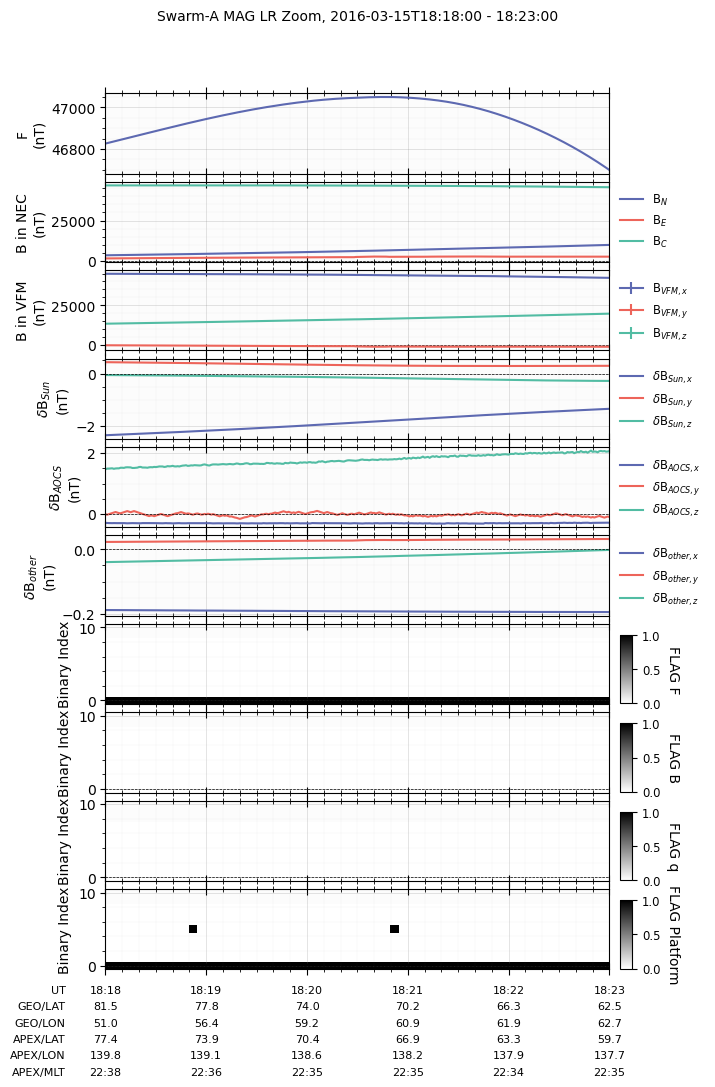
\includegraphics[width=0.7\linewidth]{files/fbdd1a64bfbcfd166df6f2202707e003.png}

\paragraph{Swarm MAG HR data}

\begin{verbatim}
def test_swarm_MAG_HR_zoom():
    """Test Swarm MAG HR data product
    
    """
    dt_fr = datetime.datetime(2016, 3, 15, 18, 18)
    dt_to = datetime.datetime(2016, 3, 15, 18, 23)

    db = dashboards.TSDashboard(
        dt_fr=dt_fr, dt_to=dt_to, figure_config={'figsize': (8, 12)},
        timeline_extra_labels=['GEO_LAT', 'GEO_LON', 'APEX_LAT', 'APEX_LON', 'APEX_MLT',]  # Not applicable for very scattered data points like AEJ_PBS peaks
        )

    ds = db.dock(datasource_contents=['esa_eo', 'swarm', 'l1b', 'mag_hr'], sat_id='A', add_APEX=True,)

    panel_layouts = [
        [ds['B_N'], ds['B_E'], ds['B_C']],
        [ds['B_VFM_x'], ds['B_VFM_y'], ds['B_VFM_z']],
        [ds['dB_Sun_VFM_x'], ds['dB_Sun_VFM_y'], ds['dB_Sun_VFM_z']],
        [ds['dB_AOCS_VFM_x'], ds['dB_AOCS_VFM_y'], ds['dB_AOCS_VFM_z']],
        [ds['dB_other_VFM_x'], ds['dB_other_VFM_y'], ds['dB_other_VFM_z']],
        [ds['FLAG_B_BIN_AUX']],
        [ds['FLAG_q_BIN_AUX']],
        [ds['FLAG_Platform_BIN_AUX']],
    ]

    db.set_layout(panel_layouts=panel_layouts)
    db.draw()
    db.add_title(title='Swarm -{} MAG HR Zoom'.format(ds.sat_id), fontsize='medium', append_time=True)
    
    db.save_figure(
        file_dir=file_dir_figure, 
        file_name='example_MAG_HR_Swarm -{}_zoom'.format(ds.sat_id), 
        dpi=100, 
        append_time=False
    )
    db.show()
test_swarm_MAG_HR_zoom()
\end{verbatim}

\begin{verbatim}
Create a new figure: Figure(800x1200).
Searching the data product "MAG_HR" with the version "latest" on the server...
INFO: Indexing the files for the product MAG_HR of the satellite A ...
The file [PosixPath('/data/afys -ionosphere/data/ESA/SWARM/Level1b/MAG_HR/0701/Sat_A/2016/SW_OPER_MAGA_HR_1B_20160315T000000_20160315T235959_0701_MDR_MAG_HR.cdf'), PosixPath('/data/afys -ionosphere/data/ESA/SWARM/Level1b/MAG_HR/0701/Sat_A/2016/SW_OPER_MAGA_HR_1B_20160315T000000_20160315T235959_0701_ASM_VFM_IC.cdf')] already exists: skip downloading.
WARNING: Multiple files found for the pattern *20160315T000000*20160315T235959*0701*.cdf in the directory /data/afys -ionosphere/data/ESA/SWARM/Level1b/MAG_HR/0701/Sat_A/2016!
\end{verbatim}

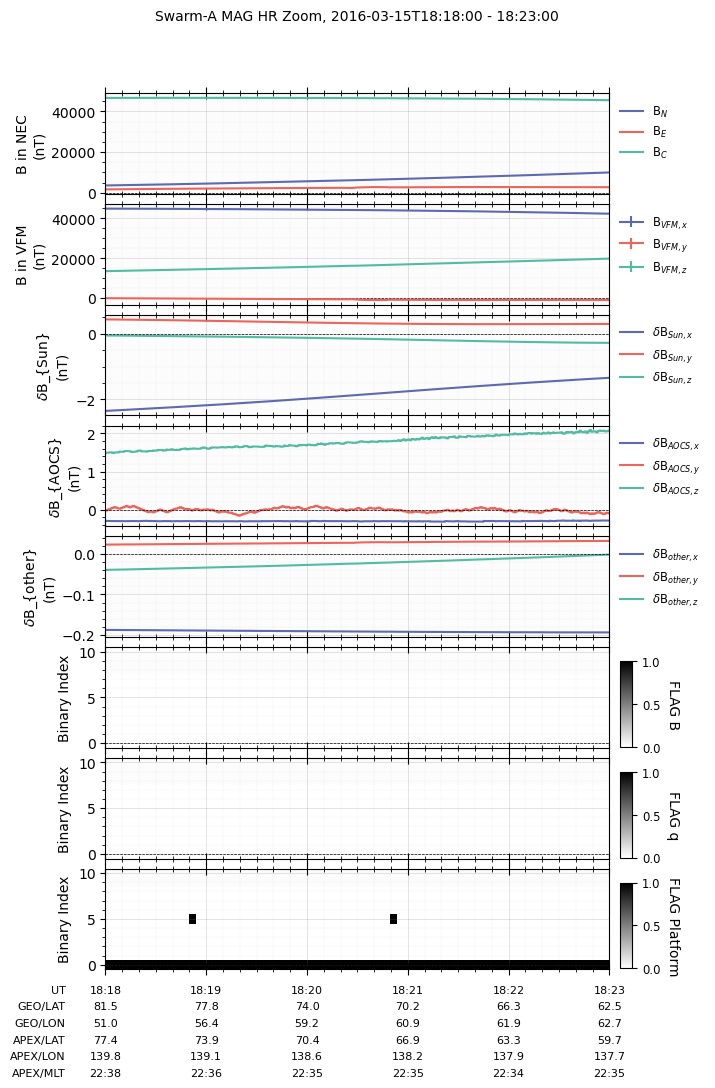
\includegraphics[width=0.7\linewidth]{files/bf8bac4495659d64665ba9d1dd6c0234.png}

\paragraph{Swarm MAG LR data from Swarm VirES service}

\subparagraph{With CHAOS modeled B-field}

\begin{verbatim}
def test_swarm_MAG_LR_from_VirES_OPER():
    """Test loading Swarm MAG LR data product from VirES

    """
    dt_fr = datetime.datetime(2016, 3, 15, 18, 18)
    dt_to = datetime.datetime(2016, 3, 15, 18, 23)

    # Default kwargs for VirES data loading, which can be overridden when calling the dock method to load data from VirES. The measurements, models, and residuals to load can be specified in the kwargs_products dictionary. The default settings are for loading all available measurements and models, and no residuals. The available measurements and models depend on the specific collection and product being loaded, and can be checked in the VirES API documentation or by inspecting the variables in the loaded dataset.
    kwargs_products_default = {
            "measurements": [
                'B_VFM', 'B_NEC', 'dB_Sun', 'dB_AOCS', 'dB_other', 'B_error',
                'q_NEC_CRF', 'Att_error',
                'Flags_B', 'Flags_q', 'Flags_Platform', 'Flags_F',
                'ASM_Freq_Dev', 'F', 'F_error', 'dF_Sun', 'dF_AOCS', 'dF_other',
            ],
            "models": [
                'CHAOS -Core',
            ],
            "residuals": False,
        }
    
    
    db = dashboards.TSDashboard(
        dt_fr=dt_fr, dt_to=dt_to, figure_config={'figsize': (8, 12)},
        timeline_extra_labels=['GEO_LAT', 'GEO_LON', 'APEX_LAT', 'APEX_LON', 'APEX_MLT',]  # Not applicable for very scattered data points like AEJ_PBS peaks
        )

    ds = db.dock(
        datasource_contents=['esa_eo', 'swarm', 'l1b', 'mag_lr'], 
        from_VirES=True, from_FAST=False,
        sat_id='A', add_APEX=True,
        kwargs_VirES={"kwargs_products": kwargs_products_default},
    )

    panel_layouts = [
        [ds['F']],
        [ds['B_N'], ds['B_E'], ds['B_C']],
        [ds['B_VFM_x'], ds['B_VFM_y'], ds['B_VFM_z']],
        [ds['dB_Sun_VFM_x'], ds['dB_Sun_VFM_y'], ds['dB_Sun_VFM_z']],
        [ds['dB_AOCS_VFM_x'], ds['dB_AOCS_VFM_y'], ds['dB_AOCS_VFM_z']],
        [ds['dB_other_VFM_x'], ds['dB_other_VFM_y'], ds['dB_other_VFM_z']],
        [ds['FLAG_F_BIN_AUX']],
        [ds['FLAG_B_BIN_AUX']],
        [ds['FLAG_q_BIN_AUX']],
        [ds['FLAG_Platform_BIN_AUX']],
    ]

    db.set_layout(panel_layouts=panel_layouts)
    db.draw()
    db.add_title(title='Swarm -{} MAG LR Zoom from VirES OPER'.format(ds.sat_id), fontsize='medium', append_time=True)
    
    db.save_figure(
        file_dir=file_dir_figure, 
        file_name='example_MAG_LR_Swarm -{}_zoom_VirES_OPER'.format(ds.sat_id), 
        dpi=100, 
        append_time=False
    )
    db.show()
test_swarm_MAG_LR_from_VirES_OPER()
\end{verbatim}

\begin{verbatim}
Create a new figure: Figure(800x1200).
INFO: Loading data from VirES for collection SW_OPER_MAGA_LR_1B with products {'measurements': ['B_VFM', 'B_NEC', 'dB_Sun', 'dB_AOCS', 'dB_other', 'B_error', 'q_NEC_CRF', 'Att_error', 'Flags_B', 'Flags_q', 'Flags_Platform', 'Flags_F', 'ASM_Freq_Dev', 'F', 'F_error', 'dF_Sun', 'dF_AOCS', 'dF_other'], 'models': ['CHAOS -Core'], 'residuals': False}.
Processing:  100%|██████████|  [ Elapsed: 00:00, Remaining: 00:00 ] [1/1] 
Downloading: 100%|██████████|  [ Elapsed: 00:00, Remaining: 00:00 ] (0.219MB)
INFO: Data loaded from VirES.
WARNING: Variable name Spacecraft not found in the variable name dictionary, and no unique match found. Skipping this variable.
WARNING: Variable SC_GEO_R is not in the default variable names and does not match the patterns for automatically assigning configured variable names. It will be added without a configured variable name, and may not be included in the default panels for plotting and analysis. Please check if this variable should be included in the default variable names or if it follows the naming patterns for automatic assignment of configured variable names.
WARNING: Variable B_NEC_CHAOS -Core is not in the default variable names and does not match the patterns for automatically assigning configured variable names. It will be added without a configured variable name, and may not be included in the default panels for plotting and analysis. Please check if this variable should be included in the default variable names or if it follows the naming patterns for automatic assignment of configured variable names.
/opt/anaconda3/envs/Swarm/lib/python3.12/site -packages/numpy/_core/numeric.py:476: RuntimeWarning: invalid value encountered in cast
  multiarray.copyto(res, fill_value, casting='unsafe')
\end{verbatim}

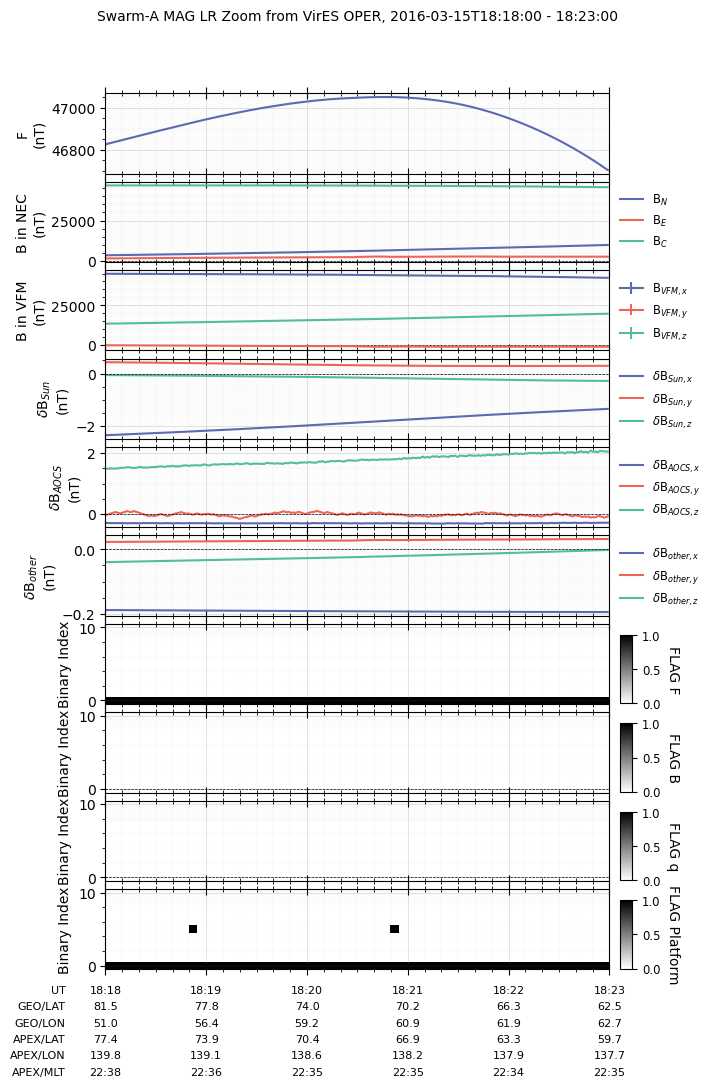
\includegraphics[width=0.7\linewidth]{files/455693ca58666f74048290f5d9079a75.png}

\subparagraph{With CHAOS modeled B-field disturbances}

\begin{verbatim}
def test_swarm_MAG_LR_from_VirES_OPER_Residuals():
    """Test loading Swarm MAG LR data product from VirES

    """
    dt_fr = datetime.datetime(2016, 3, 15, 18, 18)
    dt_to = datetime.datetime(2016, 3, 15, 18, 23)

    # Default kwargs for VirES data loading, which can be overridden when calling the dock method to load data from VirES. The measurements, models, and residuals to load can be specified in the kwargs_products dictionary. The default settings are for loading all available measurements and models, and no residuals. The available measurements and models depend on the specific collection and product being loaded, and can be checked in the VirES API documentation or by inspecting the variables in the loaded dataset.
    kwargs_products_default = {
            "measurements": [
                'B_VFM', 'B_NEC', 'dB_Sun', 'dB_AOCS', 'dB_other', 'B_error',
                'q_NEC_CRF', 'Att_error',
                'Flags_B', 'Flags_q', 'Flags_Platform', 'Flags_F',
                'ASM_Freq_Dev', 'F', 'F_error', 'dF_Sun', 'dF_AOCS', 'dF_other',
            ],
            "models": [
                'CHAOS -Core',
            ],
            "residuals": True,
        }
    
    
    db = dashboards.TSDashboard(
        dt_fr=dt_fr, dt_to=dt_to, figure_config={'figsize': (8, 12)},
        timeline_extra_labels=['GEO_LAT', 'GEO_LON', 'APEX_LAT', 'APEX_LON', 'APEX_MLT',]  # Not applicable for very scattered data points like AEJ_PBS peaks
        )

    ds = db.dock(
        datasource_contents=['esa_eo', 'swarm', 'l1b', 'mag_lr'], 
        from_VirES=True, from_FAST=False,
        sat_id='A', add_APEX=True,
        kwargs_VirES={"kwargs_products": kwargs_products_default},
    )

    panel_layouts = [
        [ds['F_res_CHAOS -Core']],
        [ds['B_res_CHAOS -Core_N'], ds['B_res_CHAOS -Core_E'], ds['B_res_CHAOS -Core_C']],
        [ds['B_VFM_x'], ds['B_VFM_y'], ds['B_VFM_z']],
        [ds['dB_Sun_VFM_x'], ds['dB_Sun_VFM_y'], ds['dB_Sun_VFM_z']],
        [ds['dB_AOCS_VFM_x'], ds['dB_AOCS_VFM_y'], ds['dB_AOCS_VFM_z']],
        [ds['dB_other_VFM_x'], ds['dB_other_VFM_y'], ds['dB_other_VFM_z']],
        [ds['FLAG_F_BIN_AUX']],
        [ds['FLAG_B_BIN_AUX']],
        [ds['FLAG_q_BIN_AUX']],
        [ds['FLAG_Platform_BIN_AUX']],
    ]

    db.set_layout(panel_layouts=panel_layouts)
    db.draw()
    db.add_title(title='Swarm -{} MAG LR Zoom from VirES OPER'.format(ds.sat_id), fontsize='medium', append_time=True)
    
    db.save_figure(
        file_dir=file_dir_figure, 
        file_name='example_MAG_LR_Swarm -{}_zoom_VirES_OPER_Residuals'.format(ds.sat_id), 
        dpi=100, 
        append_time=False
    )
    db.show()
test_swarm_MAG_LR_from_VirES_OPER_Residuals()
\end{verbatim}

\begin{verbatim}
Create a new figure: Figure(800x1200).
INFO: Loading data from VirES for collection SW_OPER_MAGA_LR_1B with products {'measurements': ['B_VFM', 'B_NEC', 'dB_Sun', 'dB_AOCS', 'dB_other', 'B_error', 'q_NEC_CRF', 'Att_error', 'Flags_B', 'Flags_q', 'Flags_Platform', 'Flags_F', 'ASM_Freq_Dev', 'F', 'F_error', 'dF_Sun', 'dF_AOCS', 'dF_other'], 'models': ['CHAOS -Core'], 'residuals': True}.
Processing:  100%|██████████|  [ Elapsed: 00:01, Remaining: 00:00 ] [1/1] 
Downloading: 100%|██████████|  [ Elapsed: 00:00, Remaining: 00:00 ] (0.202MB)
INFO: Data loaded from VirES.
WARNING: Variable name Spacecraft not found in the variable name dictionary, and no unique match found. Skipping this variable.
WARNING: Variable SC_GEO_R is not in the default variable names and does not match the patterns for automatically assigning configured variable names. It will be added without a configured variable name, and may not be included in the default panels for plotting and analysis. Please check if this variable should be included in the default variable names or if it follows the naming patterns for automatic assignment of configured variable names.
WARNING: Variable B_NEC_res_CHAOS -Core is not in the default variable names and does not match the patterns for automatically assigning configured variable names. It will be added without a configured variable name, and may not be included in the default panels for plotting and analysis. Please check if this variable should be included in the default variable names or if it follows the naming patterns for automatic assignment of configured variable names.
/opt/anaconda3/envs/Swarm/lib/python3.12/site -packages/numpy/_core/numeric.py:476: RuntimeWarning: invalid value encountered in cast
  multiarray.copyto(res, fill_value, casting='unsafe')
\end{verbatim}

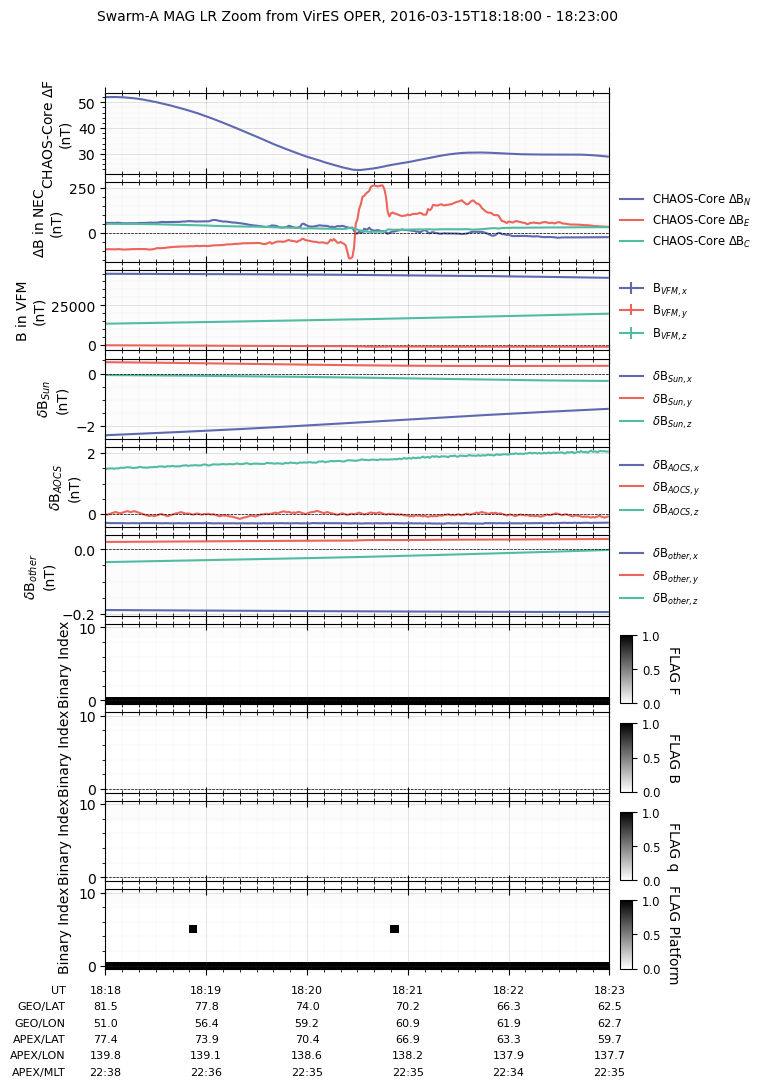
\includegraphics[width=0.7\linewidth]{files/10ae0363ce42a0130cd0276a59108004.png}

\subparagraph{Swarm MAG LR FAST data from Swarm VirES service}

\begin{verbatim}
def test_swarm_MAG_LR_from_VirES_FAST():
    """Test loading Swarm MAG LR data product from VirES

    """
    dt_fr = datetime.datetime(2026, 3, 21, 18, 00)
    dt_to = datetime.datetime(2026, 3, 21, 18, 16)

    # Default kwargs for VirES data loading, which can be overridden when calling the dock method to load data from VirES. The measurements, models, and residuals to load can be specified in the kwargs_products dictionary. The default settings are for loading all available measurements and models, and no residuals. The available measurements and models depend on the specific collection and product being loaded, and can be checked in the VirES API documentation or by inspecting the variables in the loaded dataset.
    kwargs_products_default = {
            "measurements": [
                'B_VFM', 'B_NEC', 'dB_Sun', 'dB_AOCS', 'dB_other', 'B_error',
                'q_NEC_CRF', 'Att_error',
                'Flags_B', 'Flags_q', 'Flags_Platform', 'Flags_F',
                'ASM_Freq_Dev', 'F', 'F_error', 'dF_Sun', 'dF_AOCS', 'dF_other',
            ],
            "models": [
                'CHAOS -Core',
            ],
            "residuals": False,
        }
    
    
    db = dashboards.TSDashboard(
        dt_fr=dt_fr, dt_to=dt_to, figure_config={'figsize': (8, 12)},
        timeline_extra_labels=['GEO_LAT', 'GEO_LON', 'APEX_LAT', 'APEX_LON', 'APEX_MLT',]  # Not applicable for very scattered data points like AEJ_PBS peaks
        )

    ds = db.dock(
        datasource_contents=['esa_eo', 'swarm', 'l1b', 'mag_lr'], 
        from_VirES=True, from_FAST=True,
        sat_id='A', add_APEX=True,
        kwargs_VirES={"kwargs_products": kwargs_products_default},
    )

    panel_layouts = [
        [ds['F']],
        [ds['B_N'], ds['B_E'], ds['B_C']],
        [ds['B_VFM_x'], ds['B_VFM_y'], ds['B_VFM_z']],
        [ds['dB_Sun_VFM_x'], ds['dB_Sun_VFM_y'], ds['dB_Sun_VFM_z']],
        [ds['dB_AOCS_VFM_x'], ds['dB_AOCS_VFM_y'], ds['dB_AOCS_VFM_z']],
        [ds['dB_other_VFM_x'], ds['dB_other_VFM_y'], ds['dB_other_VFM_z']],
        [ds['FLAG_F_BIN_AUX']],
        [ds['FLAG_B_BIN_AUX']],
        [ds['FLAG_q_BIN_AUX']],
        [ds['FLAG_Platform_BIN_AUX']],
    ]

    db.set_layout(panel_layouts=panel_layouts)
    db.draw()
    db.add_title(title='Swarm -{} MAG LR Zoom from VirES FAST'.format(ds.sat_id), fontsize='medium', append_time=True)
    
    db.save_figure(
        file_dir=file_dir_figure, 
        file_name='example_MAG_LR_Swarm -{}_zoom_VirES_FAST'.format(ds.sat_id), 
        dpi=100, 
        append_time=False
    )
    db.show()
test_swarm_MAG_LR_from_VirES_FAST()
\end{verbatim}

\begin{verbatim}
Create a new figure: Figure(800x1200).
INFO: Loading data from VirES for collection SW_FAST_MAGA_LR_1B with products {'measurements': ['B_VFM', 'B_NEC', 'dB_Sun', 'dB_AOCS', 'dB_other', 'B_error', 'q_NEC_CRF', 'Att_error', 'Flags_B', 'Flags_q', 'Flags_Platform', 'Flags_F', 'ASM_Freq_Dev', 'F', 'F_error', 'dF_Sun', 'dF_AOCS', 'dF_other'], 'models': ['CHAOS -Core'], 'residuals': False}.
Processing:  100%|██████████|  [ Elapsed: 00:01, Remaining: 00:00 ] [1/1] 
Downloading: 100%|██████████|  [ Elapsed: 00:00, Remaining: 00:00 ] (0.344MB)
INFO: Data loaded from VirES.
WARNING: Variable name Spacecraft not found in the variable name dictionary, and no unique match found. Skipping this variable.
WARNING: Variable SC_GEO_R is not in the default variable names and does not match the patterns for automatically assigning configured variable names. It will be added without a configured variable name, and may not be included in the default panels for plotting and analysis. Please check if this variable should be included in the default variable names or if it follows the naming patterns for automatic assignment of configured variable names.
WARNING: Variable B_NEC_CHAOS -Core is not in the default variable names and does not match the patterns for automatically assigning configured variable names. It will be added without a configured variable name, and may not be included in the default panels for plotting and analysis. Please check if this variable should be included in the default variable names or if it follows the naming patterns for automatic assignment of configured variable names.
/opt/anaconda3/envs/Swarm/lib/python3.12/site -packages/numpy/_core/numeric.py:476: RuntimeWarning: invalid value encountered in cast
  multiarray.copyto(res, fill_value, casting='unsafe')
\end{verbatim}

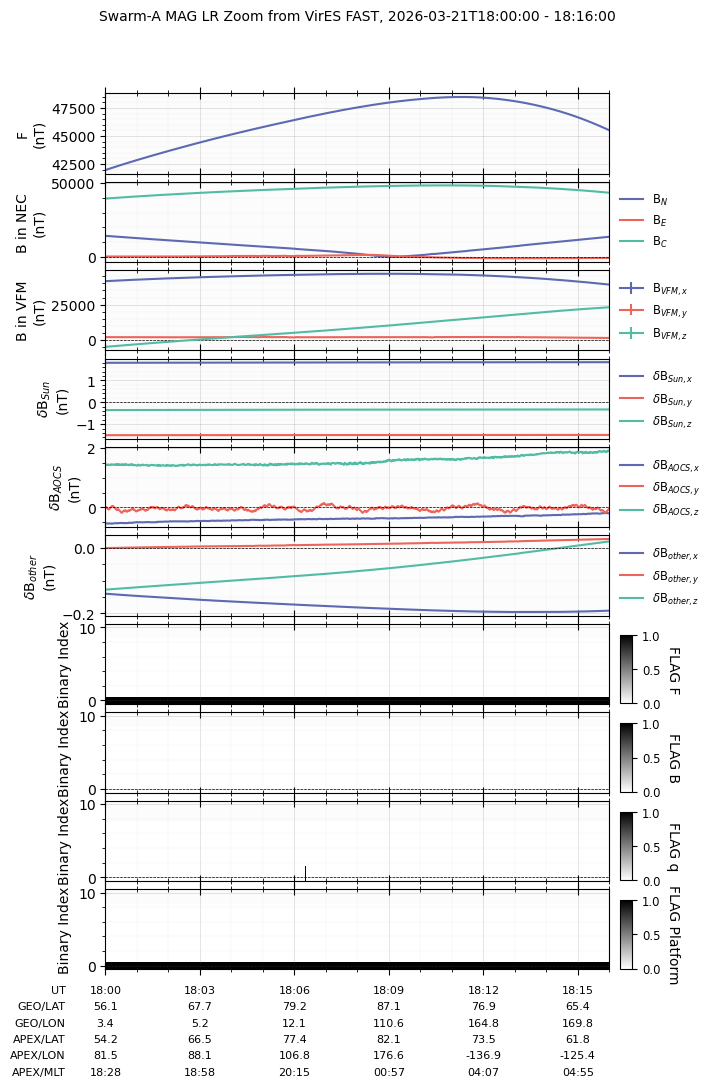
\includegraphics[width=0.7\linewidth]{files/4939f5b20234c844cd83e5b2d544119a.png}

\paragraph{Swarm MAG LR from VirES HAPI service}

\subparagraph{With CHAOS modeled B-field disturbances}

\begin{verbatim}
def test_swarm_MAG_LR_from_HAPI_OPER():
    """Test loading Swarm MAG LR data product from HAPI

    """
    dt_fr = datetime.datetime(2016, 3, 15, 18, 18)
    dt_to = datetime.datetime(2016, 3, 15, 18, 23)    
    
    db = dashboards.TSDashboard(
        dt_fr=dt_fr, dt_to=dt_to, figure_config={'figsize': (8, 12)},
        timeline_extra_labels=['GEO_LAT', 'GEO_LON', 'APEX_LAT', 'APEX_LON', 'APEX_MLT',]  # Not applicable for very scattered data points like AEJ_PBS peaks
        )

    ds = db.dock(
        datasource_contents=['esa_eo', 'swarm', 'l1b', 'mag_lr'], 
        from_HAPI=True, from_FAST=False,
        sat_id='A', add_APEX=True,
    )

    panel_layouts = [
        [ds['F']],
        [ds['F_res_Model']],
        [ds['B_N'], ds['B_E'], ds['B_C']],
        [ds['B_res_Model_N'], ds['B_res_Model_E'], ds['B_res_Model_C']],
        [ds['B_VFM_x'], ds['B_VFM_y'], ds['B_VFM_z']],
        [ds['dB_Sun_VFM_x'], ds['dB_Sun_VFM_y'], ds['dB_Sun_VFM_z']],
        [ds['dB_AOCS_VFM_x'], ds['dB_AOCS_VFM_y'], ds['dB_AOCS_VFM_z']],
        [ds['dB_other_VFM_x'], ds['dB_other_VFM_y'], ds['dB_other_VFM_z']],
        [ds['FLAG_F_BIN_AUX']],
        [ds['FLAG_B_BIN_AUX']],
        [ds['FLAG_q_BIN_AUX']],
        [ds['FLAG_Platform_BIN_AUX']],
    ]

    db.set_layout(panel_layouts=panel_layouts)
    db.draw()
    db.add_title(title='Swarm -{} MAG LR Zoom from HAPI OPER'.format(ds.sat_id), fontsize='medium', append_time=True)
    
    db.save_figure(
        file_dir=file_dir_figure, 
        file_name='example_MAG_LR_Swarm -{}_zoom_HAPI_OPER'.format(ds.sat_id), 
        dpi=100, 
        append_time=False
    )
    db.show()
test_swarm_MAG_LR_from_HAPI_OPER()
\end{verbatim}

\begin{verbatim}
Create a new figure: Figure(800x1200).
INFO: Loading data from HAPI for server https://vires.services/hapi, dataset SW_OPER_MAGA_LR_1B, parameters Timestamp,Latitude,Longitude,Radius.
INFO: Data loaded from HAPI.
INFO: Loading data from HAPI for server https://vires.services/hapi, dataset SW_OPER_MAGA_LR_1B, parameters F,dF_Sun,dF_AOCS,dF_other,F_error,B_VFM,B_NEC,dB_Sun,dB_AOCS,dB_other,B_error.
INFO: Data loaded from HAPI.
INFO: Loading data from HAPI for server https://vires.services/hapi, dataset SW_OPER_MAGA_LR_1B, parameters q_NEC_CRF,Att_error,Flags_F,Flags_B,Flags_q,Flags_Platform,ASM_Freq_Dev.
INFO: Data loaded from HAPI.
INFO: Loading data from HAPI for server https://vires.services/hapi, dataset SW_OPER_MAGA_LR_1B, parameters SyncStatus,B_NEC_Model,F_Model,F_res_Model,B_NEC_res_Model.
INFO: Data loaded from HAPI.
WARNING: Variable CDF_EPOCH is not in the default variable names and does not match the patterns for automatically assigning configured variable names. It will be added without a configured variable name, and may not be included in the default panels for plotting and analysis. Please check if this variable should be included in the default variable names or if it follows the naming patterns for automatic assignment of configured variable names.
WARNING: Variable SC_GEO_R is not in the default variable names and does not match the patterns for automatically assigning configured variable names. It will be added without a configured variable name, and may not be included in the default panels for plotting and analysis. Please check if this variable should be included in the default variable names or if it follows the naming patterns for automatic assignment of configured variable names.
WARNING: Variable B_NEC_Model is not in the default variable names and does not match the patterns for automatically assigning configured variable names. It will be added without a configured variable name, and may not be included in the default panels for plotting and analysis. Please check if this variable should be included in the default variable names or if it follows the naming patterns for automatic assignment of configured variable names.
WARNING: Variable B_NEC_res_Model is not in the default variable names and does not match the patterns for automatically assigning configured variable names. It will be added without a configured variable name, and may not be included in the default panels for plotting and analysis. Please check if this variable should be included in the default variable names or if it follows the naming patterns for automatic assignment of configured variable names.
/opt/anaconda3/envs/Swarm/lib/python3.12/site -packages/numpy/_core/numeric.py:476: RuntimeWarning: invalid value encountered in cast
  multiarray.copyto(res, fill_value, casting='unsafe')
\end{verbatim}

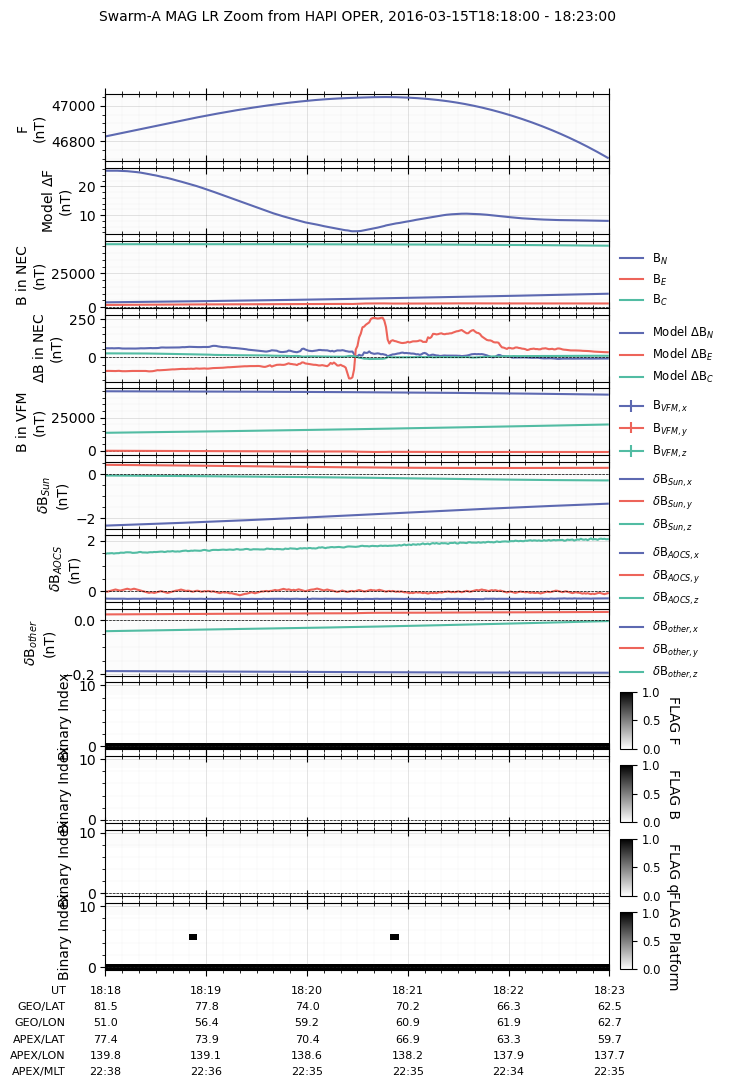
\includegraphics[width=0.7\linewidth]{files/b257be11371014259f98d2c0ca090599.png}

\subparagraph{Swarm MAG LR FAST from VirES HAPI service}

\begin{verbatim}
def test_swarm_MAG_LR_from_HAPI_FAST():
    """Test loading Swarm MAG LR data product from HAPI

    """
    dt_fr = datetime.datetime(2026, 3, 21, 18, 00)
    dt_to = datetime.datetime(2026, 3, 21, 18, 16)
    
    
    db = dashboards.TSDashboard(
        dt_fr=dt_fr, dt_to=dt_to, figure_config={'figsize': (8, 12)},
        timeline_extra_labels=['GEO_LAT', 'GEO_LON', 'APEX_LAT', 'APEX_LON', 'APEX_MLT',]  # Not applicable for very scattered data points like AEJ_PBS peaks
        )

    ds = db.dock(
        datasource_contents=['esa_eo', 'swarm', 'l1b', 'mag_lr'], 
        from_HAPI=True, from_FAST=True,
        sat_id='A', add_APEX=True,
    )

    panel_layouts = [
        [ds['F']],
        [ds['F_res_Model']],
        [ds['B_N'], ds['B_E'], ds['B_C']],
        [ds['B_res_Model_N'], ds['B_res_Model_E'], ds['B_res_Model_C']],
        [ds['B_VFM_x'], ds['B_VFM_y'], ds['B_VFM_z']],
        [ds['dB_Sun_VFM_x'], ds['dB_Sun_VFM_y'], ds['dB_Sun_VFM_z']],
        [ds['dB_AOCS_VFM_x'], ds['dB_AOCS_VFM_y'], ds['dB_AOCS_VFM_z']],
        [ds['dB_other_VFM_x'], ds['dB_other_VFM_y'], ds['dB_other_VFM_z']],
        [ds['FLAG_F_BIN_AUX']],
        [ds['FLAG_B_BIN_AUX']],
        [ds['FLAG_q_BIN_AUX']],
        [ds['FLAG_Platform_BIN_AUX']],
    ]

    db.set_layout(panel_layouts=panel_layouts)
    db.draw()
    db.add_title(title='Swarm -{} MAG LR Zoom from HAPI FAST'.format(ds.sat_id), fontsize='medium', append_time=True)
    
    db.save_figure(
        file_dir=file_dir_figure, 
        file_name='example_MAG_LR_Swarm -{}_zoom_HAPI_FAST'.format(ds.sat_id), 
        dpi=100, 
        append_time=False
    )
    db.show()
test_swarm_MAG_LR_from_HAPI_FAST()
\end{verbatim}

\begin{verbatim}
Create a new figure: Figure(800x1200).
INFO: Loading data from HAPI for server https://vires.services/hapi, dataset SW_FAST_MAGA_LR_1B, parameters Timestamp,Latitude,Longitude,Radius.
INFO: Data loaded from HAPI.
INFO: Loading data from HAPI for server https://vires.services/hapi, dataset SW_FAST_MAGA_LR_1B, parameters F,dF_Sun,dF_AOCS,dF_other,F_error,B_VFM,B_NEC,dB_Sun,dB_AOCS,dB_other,B_error.
INFO: Data loaded from HAPI.
INFO: Loading data from HAPI for server https://vires.services/hapi, dataset SW_FAST_MAGA_LR_1B, parameters q_NEC_CRF,Att_error,Flags_F,Flags_B,Flags_q,Flags_Platform,ASM_Freq_Dev.
INFO: Data loaded from HAPI.
INFO: Loading data from HAPI for server https://vires.services/hapi, dataset SW_FAST_MAGA_LR_1B, parameters SyncStatus,B_NEC_Model,F_Model,F_res_Model,B_NEC_res_Model.
INFO: Data loaded from HAPI.
WARNING: Variable CDF_EPOCH is not in the default variable names and does not match the patterns for automatically assigning configured variable names. It will be added without a configured variable name, and may not be included in the default panels for plotting and analysis. Please check if this variable should be included in the default variable names or if it follows the naming patterns for automatic assignment of configured variable names.
WARNING: Variable SC_GEO_R is not in the default variable names and does not match the patterns for automatically assigning configured variable names. It will be added without a configured variable name, and may not be included in the default panels for plotting and analysis. Please check if this variable should be included in the default variable names or if it follows the naming patterns for automatic assignment of configured variable names.
WARNING: Variable B_NEC_Model is not in the default variable names and does not match the patterns for automatically assigning configured variable names. It will be added without a configured variable name, and may not be included in the default panels for plotting and analysis. Please check if this variable should be included in the default variable names or if it follows the naming patterns for automatic assignment of configured variable names.
WARNING: Variable B_NEC_res_Model is not in the default variable names and does not match the patterns for automatically assigning configured variable names. It will be added without a configured variable name, and may not be included in the default panels for plotting and analysis. Please check if this variable should be included in the default variable names or if it follows the naming patterns for automatic assignment of configured variable names.
/opt/anaconda3/envs/Swarm/lib/python3.12/site -packages/numpy/_core/numeric.py:476: RuntimeWarning: invalid value encountered in cast
  multiarray.copyto(res, fill_value, casting='unsafe')
\end{verbatim}

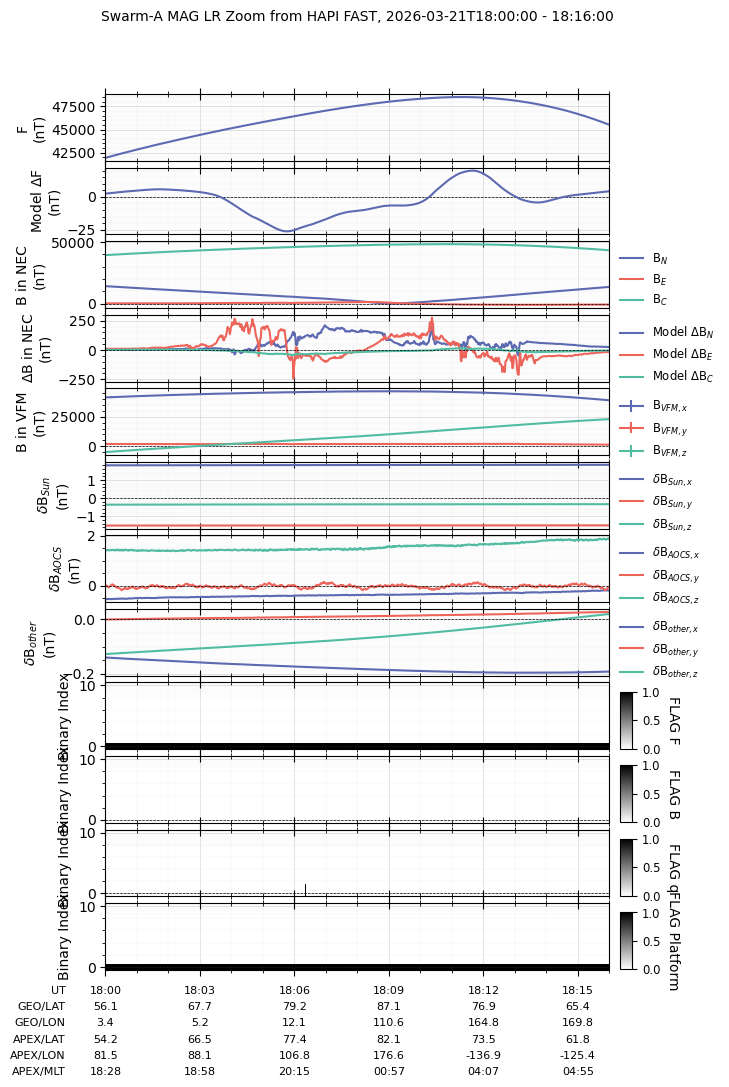
\includegraphics[width=0.7\linewidth]{files/46497c658e5cff4f2a98f37413cefedc.png}